% Bulanik Mantik donem projesi teknik raporu
% derleme: report/ klasorunde  latexmk -xelatex report.tex
\documentclass[11pt,a4paper]{article}

\usepackage{fontspec}
\usepackage{polyglossia}
\setdefaultlanguage{turkish}
\setmainfont{Latin Modern Roman}
\setmonofont{Latin Modern Mono}[Scale=0.95]
\usepackage{unicode-math}
\setmathfont{Latin Modern Math}

\usepackage[margin=2.3cm]{geometry}
\usepackage{graphicx}
\usepackage{booktabs}
\usepackage{tabularx}
\usepackage{multirow}
\usepackage{float}
\usepackage[font=small,labelfont=bf]{caption}
\usepackage{enumitem}
\usepackage{xcolor}
\usepackage{tikz}
\usetikzlibrary{positioning,arrows.meta}
\usepackage[hidelinks]{hyperref}
\usepackage{microtype}

\setlist{itemsep=1pt,topsep=3pt}
\setlength{\parskip}{3pt}
\setlength{\emergencystretch}{2.5em}
\graphicspath{{../results/figures/}}
\newcommand{\gbir}{g_1}
\newcommand{\giki}{g_2}

\title{\textbf{Yapay Bağışıklık Tabanlı IoT Saldırı Tespitinde\\ Bulanık Karar Katmanı:\\ NaIM-IDS'in Yeniden Gerçekleştirilmesi ve Genişletilmesi}}
\author{Alperen Başkaya \quad (1306220066)\\ \small Bulanık Mantık Dersi Dönem Projesi, 2026 Güz}
\date{Kasım 2026}

\begin{document}
\maketitle

\begin{abstract}
\noindent Bu çalışmada Ma ve ark.~\cite{ma2024} tarafından önerilen yapay bağışıklık tabanlı IoT saldırı tespit çerçevesinin (NaIM-IDS) tespit çekirdeği yeniden gerçekleştirilmiştir. Yeniden gerçekleştirilen kısım, Fuzzy C-Means ile self kümeleme, Red Fox Optimization ile sınır dedektörleri ve genetik algoritma ile sınır dışı dedektörlerden oluşur. Yöntem Iris, Skin ve BoT-IoT veri setlerinde makaledeki deneylerle karşılaştırılmıştır. NaIM-IDS'in Skin tespit oranı (\%98.62 / makalede \%98.55) ve BoT-IoT doğruluğu (\%98.40 / \%98.60) makaleyle 0.2 puan içinde örtüşmektedir. Özgün katkı olarak, negatif seçim dedektörlerinin keskin kararının yerine dedektör kapsaması ile self uzaklığını birleştiren 9 kurallı bir Mamdani/Sugeno çıkarım sistemi önerilmiştir. Önerilen katman Skin'de F1 değerini 99.24'ten 99.67'ye çıkarmış (Wilcoxon $p = 0.002$), BoT-IoT'de ise en yüksek AUC'yi (99.78) vermekle birlikte yanlış alarm oranını artırmıştır. Ablasyon sonuçları, FCM'nin bu uygulamada doğruluğu değil yalnızca hesap maliyetini etkilediğini göstermektedir.

\smallskip\noindent\textbf{Anahtar kelimeler:} negatif seçim algoritması, Fuzzy C-Means, Mamdani, Sugeno, IoT saldırı tespiti, BoT-IoT
\end{abstract}

%=====================================================================
\section{Giriş (Introduction)}

Nesnelerin İnterneti (IoT) cihazları sınırlı işlem gücüyle çalışır, çoğunlukla güncellenmez ve botnet saldırılarının sık hedefidir. İmza tabanlı saldırı tespit sistemleri (IDS) daha önce görülmemiş saldırıları yakalayamaz. Derin öğrenme tabanlı sistemler ise kaynak tüketimi yüksek ve kararlarını açıklaması zor modellerdir~\cite{arp2022}.

Yapay bağışıklık sistemlerindeki \emph{negatif seçim algoritması} (NSA), vücuttaki T hücrelerinin olgunlaşma sürecinden esinlenir~\cite{forrest1994}. Algoritma yalnızca normal trafikten (``self'') öğrenir. Normal bölgeye değmeyen dedektörler üretilir ve bir dedektöre düşen her örnek anomali sayılır. Gerçek değerli NSA ailesinde~\cite{gonzalez2003,ji2004} dedektörler, özellik uzayında birer hiperküredir. Bu yaklaşımın bilinen iki sorunu vardır. Rastgele üretilen dedektörler kapsanmayan boşluklar bırakır. Ayrıca her aday dedektörün bütün self örneklerle karşılaştırılması eğitim süresini uzatır.

Referans makale~\cite{ma2024} bu iki soruna karşı NaIM-IDS'i önerir. Self örnekler Fuzzy C-Means (FCM) ile kümelenir, dedektörler ise optimizasyon algoritmalarıyla uyarlanabilir biçimde üretilir. Ancak tespit kararı keskin kalır: bir örnek ya bir dedektörün içindedir ya da değildir. Kürenin hemen dışındaki bir saldırı ile normal trafiğin tam ortasındaki bir örnek aynı ``0'' kararını alır.

Bu projenin amacı, NaIM-IDS'in tespit çekirdeğini makaledeki tanımlardan yeniden gerçekleştirmek, makaledeki temel deneyleri tekrarlamak ve keskin kararı bulanık bir anomali derecesine dönüştürmenin etkisini kontrollü deneylerle ölçmektir. Katkılar şunlardır:
\begin{itemize}
  \item NaIM-IDS tespit çekirdeğinin açık kaynaklı, tekrar üretilebilir bir Python uygulaması ve 14 belgelenmiş varsayım (yazarlar kod yayımlamamıştır).
  \item Iris, Skin ve BoT-IoT üzerinde makaleyle karşılaştırmalı yeniden üretim deneyleri, veri sızıntısı kontrolü, kümeleme ablasyonu ve parametre hassasiyeti analizi.
  \item NSA dedektörlerinin geometrisinden türetilen iki girdili, 9 kurallı bir bulanık karar katmanı. Üyelik fonksiyonu türü, çıkarım yöntemi ve durulaştırma yöntemi bu katman üzerinde karşılaştırıldı.
\end{itemize}

%=====================================================================
\section{İlgili Çalışmalar (Related Work)}

\textbf{Negatif seçim algoritmaları.} Forrest ve ark.~\cite{forrest1994} NSA'yı ikili uzayda tanımlamıştır. González ve Dasgupta~\cite{gonzalez2003} algoritmayı gerçek değerli uzaya taşımış, Ji ve Dasgupta~\cite{ji2004} ise değişken yarıçaplı dedektörler kullanan V-Detector'ı önermiştir. HD-NSA~\cite{he2021} uzayı hiyerarşik olarak bölerek dedektör üretimini hızlandırır. Li ve ark.~\cite{li2025} aday dedektör merkezlerini rastgele değil, eğitimdeki anomali örneklerinden seçer; kapsanmayan boşluklara düşen örnekleri de en yakın komşu sınıflandırmasıyla ikinci bir kez değerlendirir. Gupta ve Dasgupta~\cite{gupta2021} son on yılın NSA çalışmalarını derlemiştir.

\textbf{IoT saldırı tespitinde yapay bağışıklık.} Yang ve Yang~\cite{yang2021} IoT ağ katmanı için bağışıklık tabanlı, çevrimiçi öğrenebilen bir tespit modeli önermiştir. Soni ve ark.~\cite{soni2025} klonal seçim, varyasyonel otokodlayıcı ve dendritik hücre modelini birleştiren HAIS-IDS'i altı IoT veri setinde sınamıştır. Shorman ve ark.~\cite{shorman2025} NSA, klonal seçim ve tehlike teorisini altı veri setinde karşılaştırmış; tehlike teorisi ortalama \%94.6 doğruluğa ulaşırken NSA yaklaşık \%91.8'de kalmıştır. Bejoy ve ark.~\cite{bejoy2022} genel amaçlı bir siber bağışıklık çerçevesi tanımlamıştır.

\textbf{Bulanık mantık tabanlı saldırı tespiti.} Javaheri ve ark.~\cite{javaheri2023} DDoS ve ağ anomali tespitindeki bulanık yöntemleri sınıflandıran kapsamlı bir derleme sunar. Pérez Sevilla ve ark.~\cite{perez2026} endüstriyel IoT için altı akış özelliğiyle çalışan, kural sayısı 211'den 88'e budanmış açıklanabilir bir ANFIS önermiştir. Bu çalışma F1 = 0.904 ve AUC = 0.972 değerlerine ulaşmış ve bir Mamdani baseline'ını geride bırakmıştır.

\textbf{Boşluk.} Tablo~\ref{tab:lit} incelenen çalışmaları özetler. NSA tabanlı IoT çalışmaları~\cite{ma2024,he2021,li2025,soni2025,shorman2025} dedektör kararını keskin tutar. Bulanık IDS çalışmaları~\cite{javaheri2023,perez2026} ise ham akış özelliklerinden çıkarım yapar. NSA'nın ürettiği geometrik büyüklükleri, yani dedektör kapsamasını ve self uzaklığını bulanık çıkarıma girdi olarak veren bir çalışmaya rastlanmamıştır. Bu proje bu iki hattı birleştirir.

\begin{table}[H]
\centering\small
\caption{İlgili çalışmaların karşılaştırması.}\label{tab:lit}
\begin{tabularx}{\textwidth}{@{}lXlX@{}}
\toprule
Çalışma & Yöntem & Bulanık bileşen & Veri / sonuç \\
\midrule
Ma ve ark.~\cite{ma2024} & Uyarlanabilir NSA (FCM + RFO + GA) & FCM kümeleme & BoT-IoT Acc 98.60 \\
Ji \& Dasgupta~\cite{ji2004} & V-Detector & -- & klasik baseline \\
Li ve ark.~\cite{li2025} & Anomali örneklerinden dedektör + NN & -- & NSL-KDD, UNSW-NB15 \\
Soni ve ark.~\cite{soni2025} & Klonal seçim + VAE + dendritik model & -- & 6 IoT seti, MQTT Acc 99.83 \\
Shorman ve ark.~\cite{shorman2025} & NSA / klonal / tehlike teorisi & -- & NSA ort. Acc $\approx$91.8 \\
Pérez Sevilla ve ark.~\cite{perez2026} & ANFIS, 88 kural & ANFIS, Mamdani & TON\_IoT, F1 0.904 \\
\textbf{Bu çalışma} & NaIM çekirdeği + bulanık karar & FCM + 9 kurallı FIS & Skin F1 99.24$\to$99.67 \\
\bottomrule
\end{tabularx}
\end{table}

%=====================================================================
\section{Teorik Altyapı (Theoretical Background)}

\textbf{Bulanık küme ve üyelik fonksiyonu.} Zadeh'in bulanık kümesi~\cite{zadeh1965}, her $x$ elemanına $[0,1]$ aralığında bir üyelik derecesi $\mu_A(x)$ atar. Bu çalışmada iki üyelik fonksiyonu (MF) kullanılmıştır:
\begin{equation}
\mu_{\text{tri}}(x;a,b,c)=\max\!\Big(0,\min\!\Big(\tfrac{x-a}{b-a},\tfrac{c-x}{c-b}\Big)\Big),\qquad
\mu_{\text{gauss}}(x;\bar{x},\sigma)=\exp\!\Big(-\tfrac{(x-\bar{x})^2}{2\sigma^2}\Big).
\end{equation}
\textbf{Dilsel değişken ve bulanıklaştırma.} ``Kapsama oranı'' gibi bir değişken, ``Dışarıda, Sınırda, İçeride'' gibi dilsel terimlerle ifade edilir. Bulanıklaştırma, keskin bir girdinin her terime ait üyelik derecesini hesaplama adımıdır.

\textbf{Kural tabanı ve Mamdani çıkarımı.} ``EĞER $\gbir$ $A_i$ VE $\giki$ $B_i$ İSE $y$ $C_i$'' biçimindeki $i$. kuralın ateşleme gücü $w_i=\min(\mu_{A_i}(\gbir),\mu_{B_i}(\giki))$ olarak alınır. Mamdani yönteminde~\cite{mamdani1975} her kural kendi çıktı kümesini $w_i$ seviyesinde kırpar ve kırpılmış kümeler max ile birleştirilir: $\mu_{\text{agg}}(y)=\max_i \min(w_i,\mu_{C_i}(y))$.

\textbf{Durulaştırma.} Birleşik kümeden tek bir sayı üç yöntemle elde edilmiştir. Centroid, $y^*=\int y\,\mu_{\text{agg}}(y)\,dy\,/\int\mu_{\text{agg}}(y)\,dy$ ağırlık merkezidir. Bisector, alanı ikiye bölen noktadır. MOM (mean of maximum) ise en yüksek üyelik değerini alan noktaların ortalamasıdır.

\textbf{Sugeno çıkarımı.} Takagi--Sugeno yönteminde~\cite{takagi1985} kural çıktıları bulanık küme değil fonksiyondur. Sıfırıncı derecede bu fonksiyonlar sabittir ($z_i$) ve çıktı ağırlıklı ortalamayla bulunur: $y^*=\sum_i w_i z_i/\sum_i w_i$. Durulaştırma adımı gerekmez.

\textbf{Fuzzy C-Means.} FCM~\cite{bezdek1984}, $n$ örneği $c$ kümeye bulanık olarak atar ve aşağıdaki amaç fonksiyonunu en küçükler (makale Denk.~15--17):
\begin{equation}
J_m=\sum_{i=1}^{n}\sum_{j=1}^{c}u_{ij}^{m}\lVert x_i-v_j\rVert^2,\qquad
u_{ij}=\Big[\sum_{k=1}^{c}\Big(\tfrac{\lVert x_i-v_j\rVert}{\lVert x_i-v_k\rVert}\Big)^{\frac{2}{m-1}}\Big]^{-1},\qquad
v_j=\frac{\sum_i u_{ij}^m x_i}{\sum_i u_{ij}^m}.
\end{equation}
$m>1$ bulanıklık katsayısıdır. $m\to1$ iken atamalar keskinleşir ve FCM K-means'e yaklaşır.

\textbf{Gerçek değerli negatif seçim.} Her self örnek, yarıçapı $r_s$ olan bir hiperküredir. Merkezi $c$ olan bir aday dedektörün geçerli en büyük yarıçapı $r=d_{\min}(c,\text{self})-r_s$ ile bulunur. $r>0$ ise dedektör hiçbir self örneği kapsamaz. Bir test örneği $\lVert x-c_i\rVert\le r_i$ koşulunu sağlıyorsa anomali sayılır~\cite{ji2004}.

%=====================================================================
\section{Orijinal Yöntem (Original Method)}

NaIM-IDS~\cite{ma2024} üç modülden oluşur (Şekil~\ref{fig:arch}, üst satır).

\begin{enumerate}
  \item \textbf{Çift modüllü özellik seçimi (Bölüm 3.1).} Red Fox Optimization (RFO)~\cite{polap2021} ile Harris Hawks Optimization birleştirilir. Tent kaotik haritasıyla başlatma, sinüs tabanlı atalet ağırlığı, elit bireylere dayalı diferansiyel gelişim ve karşıt tabanlı öğrenme kullanılır. Uygunluk fonksiyonu KNN hatası ile seçilen özellik oranının ağırlıklı toplamıdır.
  \item \textbf{Self örneklerin bulanık kümelenmesi (Bölüm 3.2).} Normal örnekler FCM ile kümelenir. Aday dedektör her self örnekle değil, küme merkezi ve küme boyutuyla karşılaştırılır. Küme sayısı ve $m$, iç-küme sıkılığının kümeler arası ayrıklığa oranıyla (Com/Sep) seçilir. Makalenin hassasiyet analizinde en iyi değerler $c=5$, $m=2.3$ çıkmıştır.
  \item \textbf{Uyarlanabilir dedektör üretimi (Bölüm 3.3).} Self'e yakın sınır bölgesinde dedektörlerin konumu ve yarıçapı RFO ile, çok amaçlı bir uygunlukla optimize edilir (düşük örtüşme, yüksek kapsama, self ile eşleşmeme). Bu işlem kapsama oranı 0.95'e ulaşana kadar sürer (Algoritma~1). Sınır dışındaki non-self örnekler fark eşiği $b$'ye göre alt popülasyonlara bölünür (Denk.~20) ve her alt popülasyon genetik algoritmayla (rulet seçimi, uniform çaprazlama, hızlı mutasyon~\cite{doerr2017}) evrilir.
\end{enumerate}

Makale yöntemi BoT-IoT, NSL-KDD, UNSW-NB15 ve CICIDS-2017 üzerinde değerlendirir; BoT-IoT için Acc = 98.60 ve F1 = 98.47 raporlar. AIS karşılaştırmaları ise Iris (Tablo~7) ve Skin (Tablo~8) veri setlerinde V-Detector, RNSA, GF-RNSA, BIORV-NSA ve HD-NSA ile yapılır. Makalenin yazarları kod yayımlamamıştır.

\begin{figure}[H]
\centering
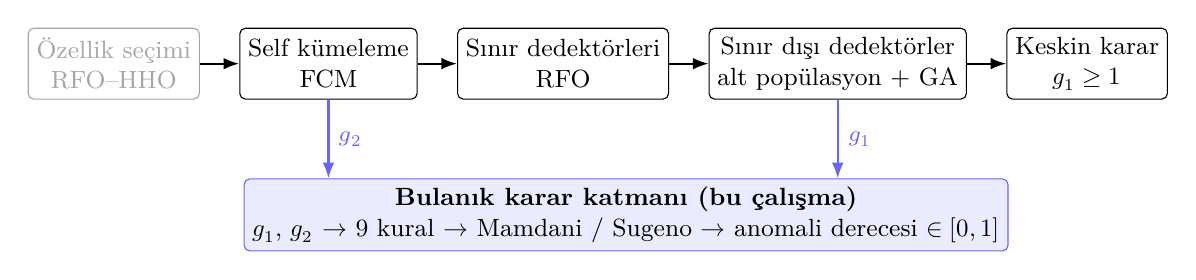
\begin{tikzpicture}[node distance=4mm and 5mm,
  box/.style={draw,rounded corners=2pt,align=center,font=\small,minimum height=9mm,inner sep=3pt},
  ours/.style={box,fill=blue!8,draw=blue!60},
  skipped/.style={box,draw=gray!70,text=gray!70},
  arr/.style={-{Latex[length=2mm]},thick}]
\node[skipped] (fs) {Özellik seçimi\\RFO--HHO};
\node[box,right=of fs] (fcm) {Self kümeleme\\FCM};
\node[box,right=of fcm] (rfo) {Sınır dedektörleri\\RFO};
\node[box,right=of rfo] (ga) {Sınır dışı dedektörler\\alt popülasyon + GA};
\node[box,right=of ga] (crisp) {Keskin karar\\$\gbir \ge 1$};
\draw[arr] (fs)--(fcm); \draw[arr] (fcm)--(rfo); \draw[arr] (rfo)--(ga); \draw[arr] (ga)--(crisp);
\node[ours,below=10mm of rfo,xshift=8mm] (fis) {\textbf{Bulanık karar katmanı (bu çalışma)}\\ $\gbir$, $\giki$ $\to$ 9 kural $\to$ Mamdani / Sugeno $\to$ anomali derecesi $\in[0,1]$};
\draw[arr,blue!60] (ga.south) -- (ga.south |- fis.north) node[midway,right,font=\footnotesize]{$\gbir$};
\draw[arr,blue!60] (fcm.south) -- (fcm.south |- fis.north) node[midway,right,font=\footnotesize]{$\giki$};
\end{tikzpicture}
\caption{NaIM-IDS ve bu çalışmanın kapsamı. Gri kutu yeniden gerçekleştirilmedi. Mavi kutu önerilen genişlemedir: $\gbir$ dedektörlerden, $\giki$ FCM'li self uzayından gelir.}\label{fig:arch}
\end{figure}

%=====================================================================
\section{Yeniden Gerçekleştirme Yöntemi (Reproduction Methodology)}

\textbf{Kapsam (MRR).} Makalenin bulanık bileşeni FCM, ana katkısı ise uyarlanabilir dedektör üretimidir. Bu nedenle yeniden gerçekleştirme bu ikisini kapsar (Şekil~\ref{fig:arch}). Özellik seçimi kapsam dışında bırakılmıştır. Makalenin kendi ablasyonuna göre (Tablo~9) bu modülün katkısı yaklaşık 0.7 puan doğruluktur. IDS veri setlerinde özellik kümesi olarak makalenin Tablo~3 listesi ve sızıntısız bir alternatif kullanılmıştır. Baseline, V-Detector'dır~\cite{ji2004}.

\textbf{Uygulama.} Kodun tamamı Python 3 ve NumPy ile sıfırdan yazıldı; FCM ve bulanık çıkarım için kütüphane kullanılmadı. Modüller şunlardır: \texttt{fcm.py} (Denk.~15--19), \texttt{detectors.py} (self uzayı ve dedektör kümesi), \texttt{rfo.py}, \texttt{ga.py}, \texttt{naim.py} ve baseline için \texttt{vdetector.py}.

\textbf{FCM ile tolerans hesabı.} Makale, aday dedektörün ``küme merkezi ve boyutu ile'' karşılaştırıldığını söyler ama bu karşılaştırmanın biçimini vermez. Bu uygulamada küme yarıçapı $R_k=\max_{s\in k}\lVert s-v_k\rVert$ olarak tanımlandı. Üçgen eşitsizliğine göre $k$ kümesindeki her $s$ için $\lVert x-s\rVert\ge\lVert x-v_k\rVert-R_k$ olur. Bu alt sınır o ana kadar bulunan en iyi uzaklıktan büyükse kümenin üyelerine hiç bakılmaz. Böylece sonuç kaba kuvvet aramasıyla \emph{birebir aynı} kalır; yalnızca hesaplanan uzaklık sayısı azalır.

\textbf{Varsayımlar.} Makalenin vermediği 14 ayrıntı varsayımla dolduruldu ve repodaki \texttt{docs} klasöründe, \texttt{ASSUMPTIONS.md} dosyasında listelendi. Sonuçları en çok etkileyenler Tablo~\ref{tab:assume}'de verilmiştir.

\begin{table}[H]
\centering\small
\caption{Sonuçları en çok etkileyen yeniden gerçekleştirme varsayımları.}\label{tab:assume}
\begin{tabularx}{\textwidth}{@{}lXX@{}}
\toprule
Konu & Makalede & Bu çalışmada \\
\midrule
Self yarıçapı $r_s$ & verilmemiş & $r_s=0.05$ ($[0,1]$ ölçeğinde) \\
Sınır bölgesi & şekille anlatılmış & self'e en yakın \%30'luk non-self dilimi \\
Dedektör uygunluğu & ``kaynak [45]'' & $F=\text{kapsama}+0.5\,r/\sqrt{d}-0.3\,\text{örtüşme}$ \\
Com/Sep indeksi & iki küme için yazılmış & $c$ kümeye genelleştirildi; $c$ ile seçildi, $m=2.3$ sabit tutuldu (indeks her zaman en büyük $m$'yi seçiyor) \\
Skin eğitim oranı & verilmemiş & her sınıftan \%2, test geri kalan $\approx$240 bin örnek \\
BoT-IoT örneklemi & verilmemiş & 477 normalin tamamı + kategoriye orantılı 5.050 saldırı \\
\bottomrule
\end{tabularx}
\end{table}

%=====================================================================
\section{Önerilen Geliştirme (Proposed Extension)}

\textbf{Gerekçe.} Keskin NSA kararı iki tür bilgiyi kullanmaz. Birincisi, bir örneğin dedektör sınırına ne kadar yakın olduğu; ikincisi, normal trafiğe ne kadar uzak olduğu. Kapsanmayan boşluklara düşen bir saldırı normal bölgeden uzakta olabilir. Dedektör sınırına yeni girmiş bir örnek ise normal trafiğin hemen kıyısında durabilir. Önerilen katman bu iki bilgiyi bir anomali derecesinde birleştirir. Böylece (i) eşik, ağın yanlış alarm toleransına göre ayarlanabilir ve ROC/AUC hesaplanabilir, (ii) dedektör boşlukları için ikinci bir kanıt kaynağı oluşur, (iii) her karar kural tablosu üzerinden açıklanabilir.

\textbf{Girdiler.} Eğitilmiş NaIM dedektörleri $\{(c_i,r_i)\}$ ve FCM'li self uzayı kullanılarak her örnek için iki girdi hesaplanır:
\begin{equation}
\gbir(x)=\min\!\Big(2,\ \max_i \frac{r_i}{\lVert x-c_i\rVert}\Big),\qquad
\giki(x)=\min\!\Big(2,\ \frac{d_{\min}(x,\text{self})}{d_{\text{ref}}}\Big).
\end{equation}
$\gbir\ge1$ olması, örneğin en az bir dedektörün içinde olduğu anlamına gelir; keskin karar tam olarak $\gbir\ge1$ eşiğidir. $d_{\text{ref}}$, eğitim saldırılarının self'e uzaklıklarının medyanıdır; test verisinden bilgi kullanılmaz.

\textbf{Üyelik fonksiyonları ve kural tabanı.} Üçgen MF parametreleri Tablo~\ref{tab:mf}'de, kural tabanı Tablo~\ref{tab:rules}'da verilmiştir. Gauss MF'lerin merkezleri üçgenlerin tepe noktalarına konmuş, $\sigma$ değerleri ise üçgenle aynı noktalarda yaklaşık 0.5 üyelik verecek şekilde seçilmiştir (Şekil~\ref{fig:mf}). Kural tabanının mantığı şudur: kürenin derin içinde ve self'ten uzak olan örnek Saldırı, kürenin dışında ve self'e yakın olan Normal sayılır. Karışık durumlar Şüpheli'dir.

\begin{table}[H]
\centering\small
\begin{minipage}[t]{0.55\textwidth}\centering
\caption{Üçgen MF parametreleri $(a,b,c)$.}\label{tab:mf}
\begin{tabular}{@{}lll@{}}
\toprule
Değişken & Terim & $(a,b,c)$ \\
\midrule
\multirow{3}{*}{$\gbir\in[0,2]$} & Dışarıda & (0, 0, 0.8) \\ & Sınırda & (0.6, 1.0, 1.4) \\ & İçeride & (1.2, 2.0, 2.0) \\
\midrule
\multirow{3}{*}{$\giki\in[0,2]$} & Yakın & (0, 0, 0.5) \\ & Orta & (0.2, 0.7, 1.2) \\ & Uzak & (0.9, 2.0, 2.0) \\
\midrule
\multirow{3}{*}{$y\in[0,1]$} & Normal & (0, 0, 0.4) \\ & Şüpheli & (0.2, 0.5, 0.8) \\ & Saldırı & (0.6, 1.0, 1.0) \\
\bottomrule
\end{tabular}
\end{minipage}\hfill
\begin{minipage}[t]{0.42\textwidth}\centering
\caption{Kural tabanı (K1--K9, VE = min).}\label{tab:rules}
\begin{tabular}{@{}llll@{}}
\toprule
$\gbir$ \textbackslash{} $\giki$ & Yakın & Orta & Uzak \\
\midrule
Dışarıda & Normal & Normal & Şüpheli \\
Sınırda & Normal & Şüpheli & Saldırı \\
İçeride & Şüpheli & Saldırı & Saldırı \\
\bottomrule
\end{tabular}
\par\medskip\raggedright\small Sugeno sabitleri: Normal $z=0$, Şüpheli $z=0.5$, Saldırı $z=1$.
\end{minipage}
\end{table}

\begin{figure}[H]
\centering
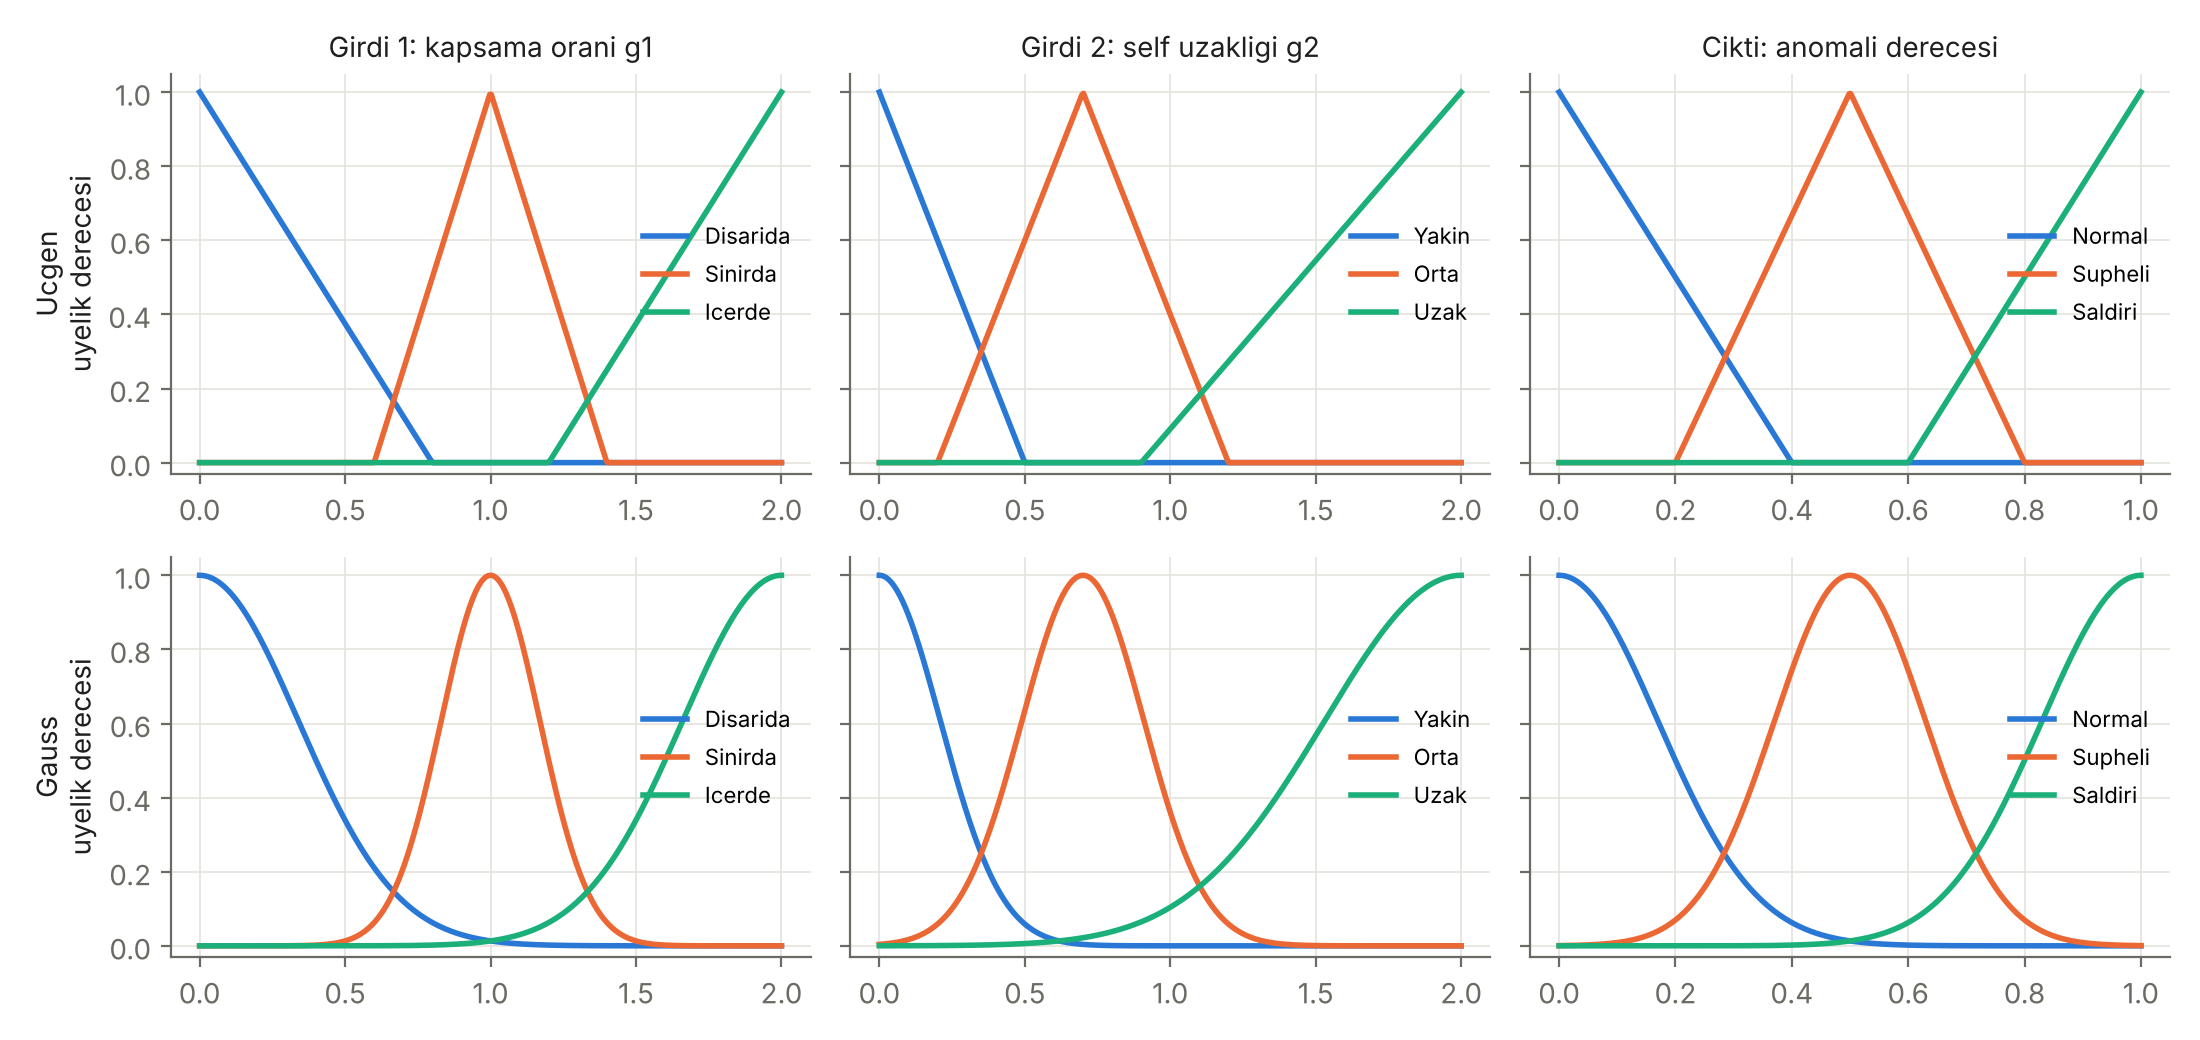
\includegraphics[width=\textwidth]{fis_membership.png}
\caption{Üçgen (üst) ve Gauss (alt) üyelik fonksiyonları.}\label{fig:mf}
\end{figure}

\textbf{Çıkarım örneği.} $\gbir=1.1$ ve $\giki=0.4$ olan bir örnek kürenin içindedir; keskin sistem ``Saldırı'' der. Bulanıklaştırmada Sınırda = 0.75, Yakın = 0.20 ve Orta = 0.40 bulunur. K5 (Sınırda VE Orta $\to$ Şüpheli) $w=0.40$, K4 (Sınırda VE Yakın $\to$ Normal) $w=0.20$ ile ateşlenir. Centroid 0.425 verir ve örnek ``Normal'' sayılır (Şekil~\ref{fig:demo}). Bu çıktı repodaki \texttt{demo.py} ile canlı olarak üretilebilir.

\begin{figure}[H]
\centering
\begin{minipage}[c]{0.52\textwidth}\centering
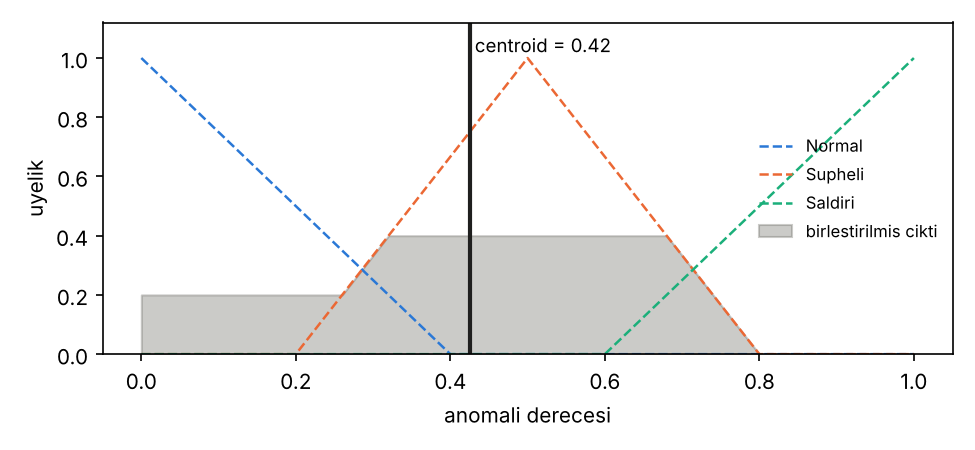
\includegraphics[width=\textwidth]{demo_inference.png}
\end{minipage}\hfill
\begin{minipage}[c]{0.44\textwidth}\centering
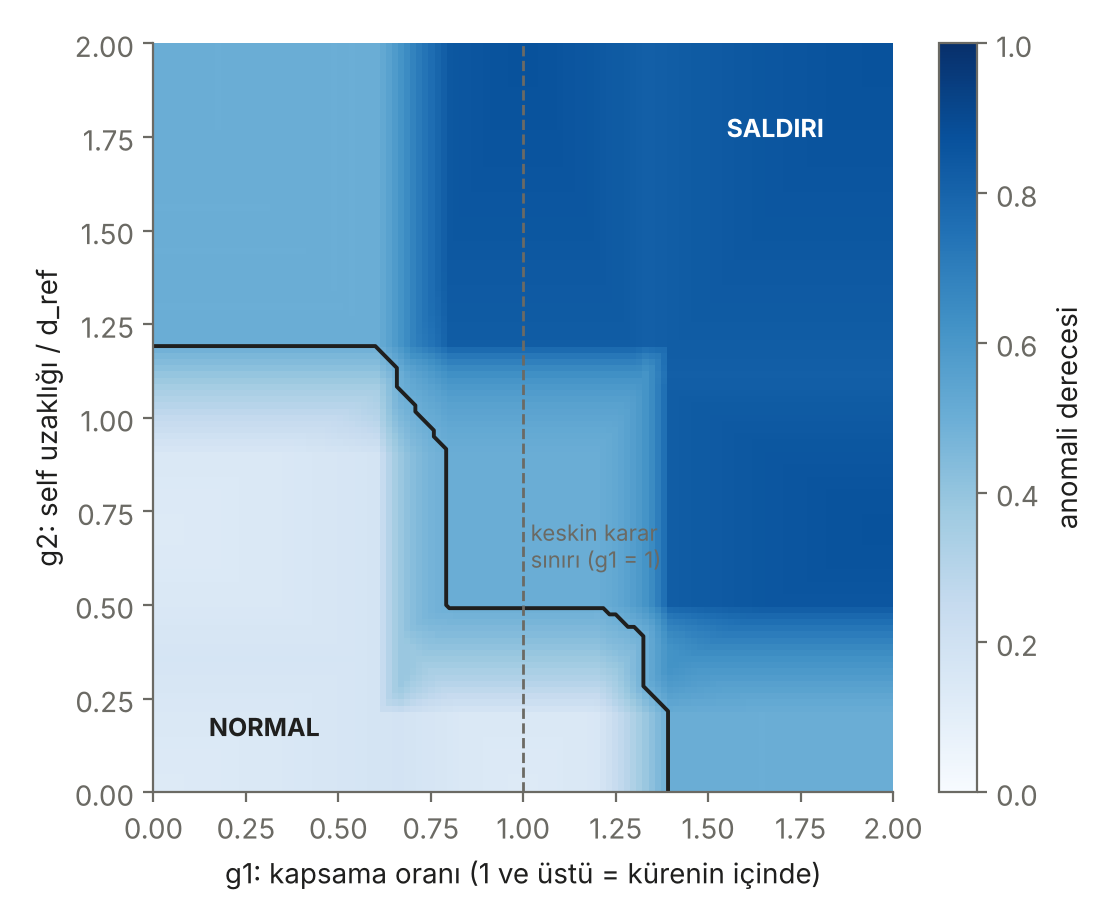
\includegraphics[width=\textwidth]{fis_surface.png}
\end{minipage}
\caption{Sol: $\gbir=1.1$, $\giki=0.4$ için Mamdani çıkarımı; kırpılmış kümelerin birleşimi ve centroid. Sağ: kontrol yüzeyi; siyah çizgi 0.5 eşiğindeki karar sınırı, kesikli çizgi keskin kararın sınırıdır.}\label{fig:demo}
\end{figure}

\textbf{Eşik seçimi ve adil karşılaştırma.} Her tekrarda eğitim kısmı 70/30 bölünür. NaIM dedektörleri \%70'lik kısımda eğitilir, eşik ise \%30'luk doğrulama kısmında F1'i en büyük yapacak şekilde seçilir. Keskin karar ve FIS \emph{aynı} dedektörleri kullanır. FIS'in kendi katkısını ayırmak için aynı eşik ayarı, FIS'siz ham kapsama skoruna ($\gbir$) da uygulanır. Karşılaştırılan varyantlar: üçgen ve Gauss MF; Mamdani ve Sugeno; centroid, bisector ve MOM; sabit (0.5) ve ayarlanmış eşik.

%=====================================================================
\section{Deney Düzeni (Experimental Setup)}

\textbf{Veri setleri.} \emph{Iris}: 150 örnek, 4 özellik; her sınıf sırayla self kabul edilir (makale Tablo~7). \emph{Skin Segmentation} (UCI): 245.057 piksel, 3 özellik (B, G, R); deri pikselleri self'tir (Tablo~8). \emph{BoT-IoT}~\cite{koroniotis2019}: resmî \%5 alt kümede 3.668.522 akış vardır ve bunların yalnızca 477'si normaldir. Bütün normaller ile kategoriye orantılı 5.050 saldırı (DDoS, DoS, keşif, hırsızlık) alınmıştır. İki özellik kümesi kullanılmıştır: makalenin Tablo~3'teki 6 özelliği ve veri seti yazarlarının ``10 best'' listesinden sıra numarası \texttt{seq} çıkarılarak elde edilen 9 özellik (``temiz''). Tüm veriler makaledeki gibi tekrar ve eksik değerlerden temizlenmiş, kategorikler LabelEncoder ile kodlanmış ve min--max ile $[0,1]$ aralığına ölçeklenmiştir.

\textbf{Deneyler.} E1: Iris, \%50 ve \%100 eğitim, 20 tekrar, test tüm veri üzerinde (makale düzeni). E2: Skin, \%2 eğitim, 10 tekrar. E3: BoT-IoT, \%50 eğitim / \%50 test, iki özellik kümesi, 10 tekrar. E4/E5: keskin karar ve FIS varyantlarının karşılaştırması, ayrık test, Iris (3 sınıf $\times$ 20 tekrar) ile Skin ve BoT-IoT (10'ar tekrar). E6: kümeleme ablasyonu (FCM, K-means, kümeleme yok; $c=5$). E7: test verisine $\sigma\in\{0,0.02,0.05,0.08,0.12\}$ Gauss gürültüsü. E8: $c$, $m$, $b$ ve $r_s$ için tek parametreli tarama, 5 tekrar.

\textbf{Parametreler.} $r_s=0.05$, $m=2.3$, $c$ Com/Sep ile $\{2,\dots,10\}$ arasından seçilir, $b=0.15$, hedef kapsama 0.95. RFO: 20 birey, 15 iterasyon. GA: 20 birey, 15 nesil, 12 bit/boyut, $p_c=0.9$. V-Detector: $c_0=0.99$.

\textbf{Ölçütler ve istatistik.} Pozitif sınıf saldırıdır. Tespit oranı DR = TP/(TP+FN), yanlış alarm oranı FAR = FP/(FP+TN), ayrıca accuracy, precision, F1, ROC-AUC, dedektör sayısı, eğitim süresi ve örnek başına test süresi ölçülmüştür. Yöntemler, aynı bölünmeler üzerinde Wilcoxon işaretli sıra testiyle karşılaştırılmıştır. 10 tekrarda bu testin verebileceği en küçük çift yönlü $p$ değeri 0.002'dir.

\textbf{Ortam.} Python 3.13, NumPy 2.5, SciPy 1.18, scikit-learn 1.9, pandas 3.0, matplotlib 3.11; 2 çekirdekli Intel Xeon 2.1 GHz, 8 GB bellek. Tüm deneyler sabit tohumlarla çalışır. Repo temiz bir ortamda klonlanıp yeniden çalıştırıldığında tablolar, süre sütunları dışında birebir aynı çıkmıştır.

%=====================================================================
\section{Sonuçlar (Results)}

\subsection{Yeniden üretim deneyleri}

Tablo~\ref{tab:e1} Iris sonuçlarını makaleyle karşılaştırır. NaIM-IDS, V-Detector'a göre yanlış alarm oranını \%50 eğitimde 2--4 kat düşürmüştür; bu, makaledeki ana örüntüyle uyumludur. Tespit oranımız Versicolor ve Virginica'da makaleden 3--4 puan düşüktür. Dedektör sayımız ise iki mertebe azdır.

\begin{table}[H]
\centering\small
\caption{E1: Iris, \%50 eğitim, 20 tekrar ortalaması (bizim / makale Tablo 7).}\label{tab:e1}
\begin{tabular}{@{}llccc@{}}
\toprule
Self & Algoritma & DR \% & FAR \% & Dedektör sayısı \\
\midrule
\multirow{2}{*}{Setosa} & V-Detector & 100.0 / 100.0 & 3.3 / 3.2 & 13.2 / 3653.1 \\
 & NaIM-IDS & 99.9 / 100.0 & 0.3 / 3.6 & 1.4 / 151.0 \\
\multirow{2}{*}{Versicolor} & V-Detector & 94.5 / 96.5 & 10.8 / 8.6 & 47.0 / 3568.4 \\
 & NaIM-IDS & 95.8 / 99.5 & 4.5 / 3.3 & 5.7 / 260.3 \\
\multirow{2}{*}{Virginica} & V-Detector & 97.8 / 96.4 & 17.9 / 10.0 & 54.9 / 2822.3 \\
 & NaIM-IDS & 96.7 / 99.6 & 4.5 / 7.8 & 5.1 / 408.0 \\
\bottomrule
\end{tabular}
\end{table}

Tablo~\ref{tab:e23}'te Skin ve BoT-IoT sonuçları verilmiştir. NaIM-IDS'in Skin tespit oranı (98.62) ve BoT-IoT doğruluğu (98.40) makaleyle 0.2 puan içinde örtüşür. BoT-IoT'de NaIM, V-Detector'ı makale özellikleriyle 6, temiz özelliklerle 21 puan geride bırakır. Makalenin seçtiği zaman damgası ve port alanları çıkarıldığında NaIM'in sonucu değişmemektedir.

\begin{table}[H]
\centering\small
\caption{E2 ve E3: Skin ve BoT-IoT, 10 tekrar ortalaması.}\label{tab:e23}
\begin{tabular}{@{}llcccc@{}}
\toprule
Veri & Algoritma & DR \% & FAR \% & Accuracy \% & F1 \% \\
\midrule
Skin & V-Detector (bizim / makale) & 98.60 / 87.20 & 0.03 / 3.04 & 98.89 & 99.29 \\
Skin & NaIM-IDS (bizim / makale) & 98.62 / 98.55 & 0.01 / 3.01 & 98.91 & 99.30 \\
\midrule
BoT-IoT & NaIM-IDS (makale) & 97.73 & -- & 98.60 & 98.47 \\
BoT-IoT, makale öz. & V-Detector & 91.53 & 0.38 & 92.23 & 95.36 \\
BoT-IoT, makale öz. & NaIM-IDS & 98.28 & 0.38 & 98.40 & 99.12 \\
BoT-IoT, temiz öz. & V-Detector & 75.29 & 1.04 & 77.15 & 84.85 \\
BoT-IoT, temiz öz. & NaIM-IDS & 98.36 & 1.14 & 98.40 & 99.12 \\
\bottomrule
\end{tabular}
\end{table}

\textbf{Kümeleme ablasyonu (E6).} FCM, tolerans aşamasındaki uzaklık hesabını Skin'de 17.03 milyondan 7.85 milyona (\%54), BoT-IoT'de 2.12 milyondan 1.44 milyona (\%32) indirmiştir. F1 ise değişmemiştir: Skin'de FCM ile 99.24, K-means ile 99.29, kümelemesiz 99.33; BoT-IoT'de FCM ile 99.19, kümelemesiz 99.17. FCM ile K-means arasında belirgin bir fark yoktur.

\textbf{Parametre hassasiyeti (E8).} Şekil~\ref{fig:e8}'de görüldüğü gibi $c$ ve $b$, F1'i 0.3 puanın içinde değiştirir ve bu değişim standart sapma bandının içinde kalır. En yüksek ortalama $c=5$'te elde edilmiştir; makale de $S=5$'i en iyi bulmuştur. $m$ doğruluğu hiç değiştirmez. En etkili parametre $r_s$'tir: $r_s=0.01$'de FAR 1.71, $r_s=0.12$'de 0.47'dir. Skin'de $c$, 2'den 10'a çıktıkça uzaklık hesabı 13.5 milyondan 5.4 milyona düşmektedir.

\begin{figure}[H]
\centering
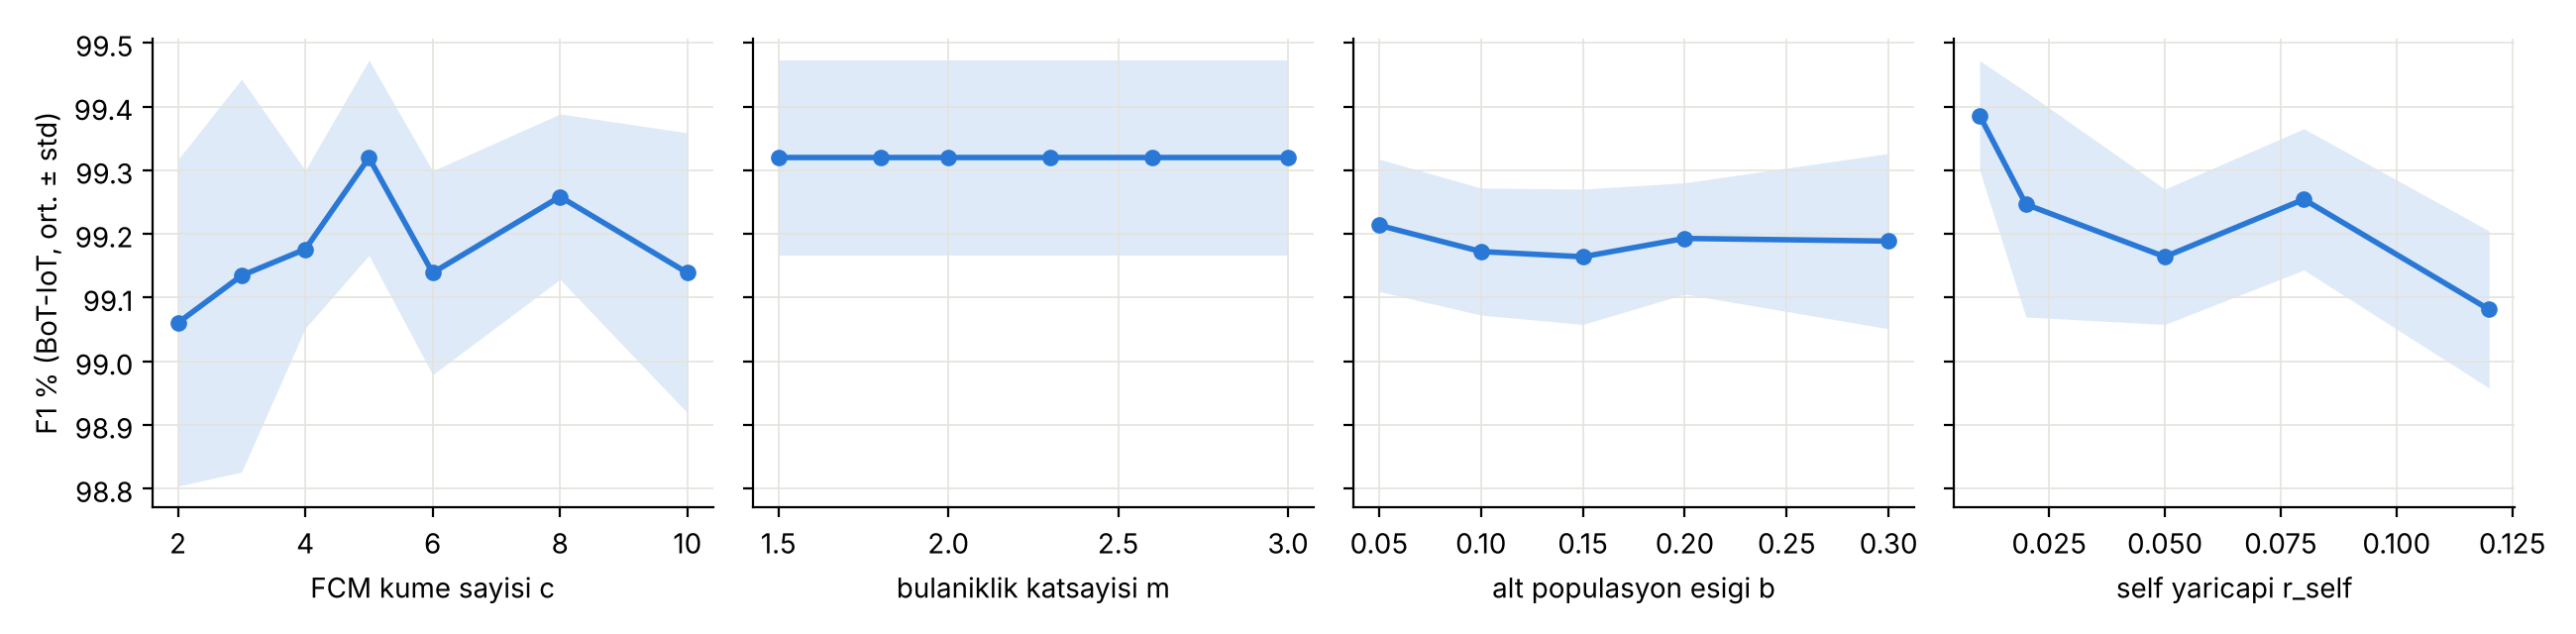
\includegraphics[width=\textwidth]{e8_sensitivity.png}
\caption{E8: BoT-IoT'de parametrelerin F1'e etkisi (5 tekrar, ortalama $\pm$ standart sapma). Dikey eksen 98.8--99.5 aralığında yakınlaştırılmıştır.}\label{fig:e8}
\end{figure}

\subsection{Bulanık karar katmanı}

Tablo~\ref{tab:e4} ana karşılaştırmayı verir. Ayarlanmış eşikte Mamdani FIS, Skin'de keskin karara göre F1'i 0.43 puan, DR'yi 0.86 puan artırır (her ikisi için $p=0.002$). FAR'daki 0.03 puanlık artış anlamlı değildir ($p=0.22$). FIS, eşiği aynı şekilde ayarlanmış FIS'siz skoru da geçer: F1 $+0.11$ ($p=0.027$), FAR $-0.19$ ($p=0.004$). BoT-IoT'de Gauss Sugeno F1'i 0.29 puan ($p=0.020$) ve DR'yi 1.03 puan ($p=0.006$) artırır, en yüksek AUC'yi verir (99.78; FIS'siz skora göre $+0.51$, $p=0.002$). Buna karşın FAR 1.71'den 7.20'ye çıkar. Sabit 0.5 eşiğinde FIS temkinli davranır: BoT-IoT'de FAR'ı 1.71'den 0.71'e indirir ($p=0.016$), ancak DR 3.39 puan düşer.

\begin{table}[H]
\centering\small
\caption{E4/E5: keskin karar ve bulanık katman (ayrık test; Skin ve BoT-IoT 10 tekrar, Iris 60 deneme). Aksi belirtilmedikçe eşik doğrulamada seçilmiştir.}\label{tab:e4}
\begin{tabular}{@{}llcccc@{}}
\toprule
Veri & Yöntem & DR \% & FAR \% & F1 \% & AUC \% \\
\midrule
\multirow{5}{*}{Skin} & Keskin (makale) & 98.49 & 0.01 & 99.24 & 99.24 \\
 & Kapsama skoru, FIS yok & 99.19 & 0.23 & 99.56 & 99.84 \\
 & FIS üçgen Mamdani centroid & \textbf{99.36} & 0.04 & \textbf{99.67} & 99.52 \\
 & FIS Gauss Mamdani centroid & 99.39 & 0.11 & 99.68 & 99.74 \\
 & FIS Gauss Sugeno & 99.58 & 0.78 & 99.69 & 99.99 \\
\midrule
\multirow{6}{*}{BoT-IoT} & Keskin (makale) & 98.60 & 1.71 & 99.22 & 98.45 \\
 & Kapsama skoru, FIS yok & 99.00 & 2.61 & 99.39 & 99.26 \\
 & FIS üçgen Mamdani centroid & 98.56 & 5.26 & 99.05 & 99.08 \\
 & FIS üçgen Mamdani MOM & 97.24 & 6.40 & 98.33 & 98.58 \\
 & FIS Gauss Sugeno & \textbf{99.63} & 7.20 & \textbf{99.51} & \textbf{99.78} \\
 & FIS üçgen Mamdani, eşik 0.5 & 95.21 & \textbf{0.71} & 97.51 & 99.08 \\
\midrule
\multirow{2}{*}{Iris} & Keskin (makale) & 94.8 & 5.0 & 96.1 & 94.9 \\
 & FIS üçgen Mamdani, eşik 0.5 & 83.1 & 0.9 & 89.6 & 96.7 \\
\bottomrule
\end{tabular}
\end{table}

Şekil~\ref{fig:roc}, ilk tekrar için ROC eğrilerini gösterir. Keskin karar tek bir çalışma noktasıdır ve bu nokta, BoT-IoT'de FIS'siz kapsama skorunun eğrisinin üzerine düşer. Çünkü keskin karar bu skorun $\gbir\ge1$ eşiğidir. BoT-IoT'de FAR'ın yaklaşık \%6'nın altında kaldığı bölgede ham kapsama skoru her iki FIS'ten de üstündür. Gauss Sugeno ancak bu değerin üzerinde öne geçer.

\begin{figure}[H]
\centering
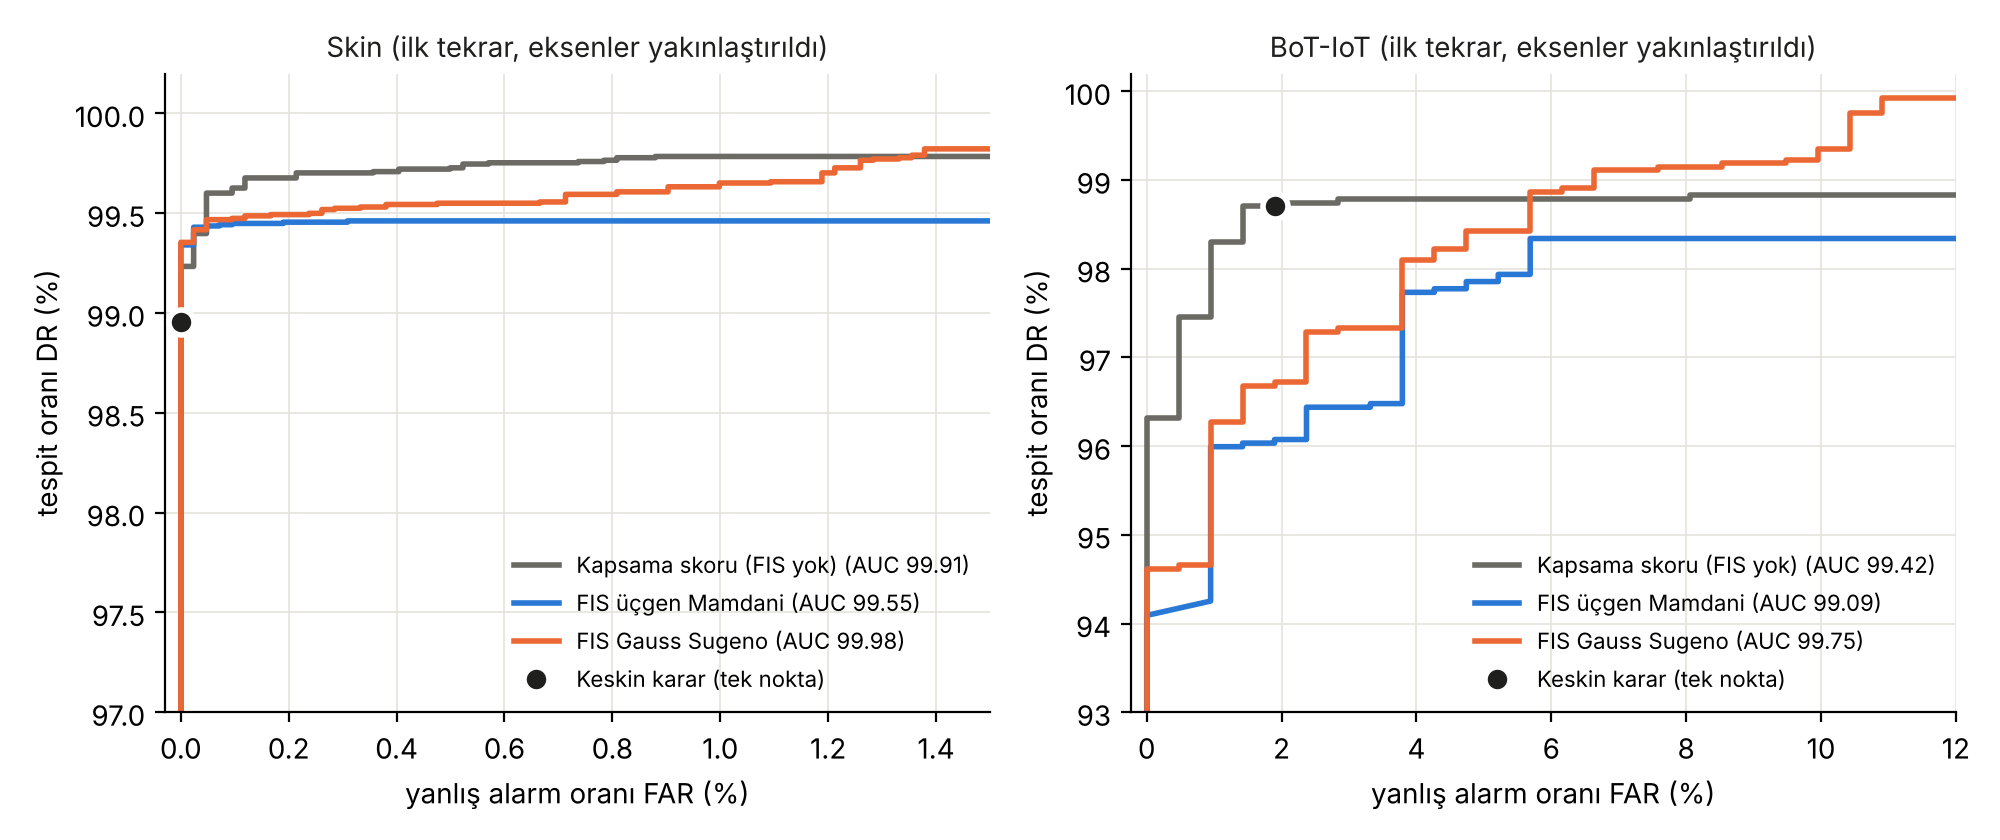
\includegraphics[width=\textwidth]{roc_curves.png}
\caption{ROC eğrileri (ilk tekrar, eksenler yakınlaştırılmış). Siyah nokta keskin kararın çalışma noktasıdır.}\label{fig:roc}
\end{figure}

Üyelik fonksiyonu ve durulaştırma karşılaştırmasında Gauss MF, her veri setinde üçgen MF'den daha yüksek AUC vermiştir (Skin 99.74 / 99.52, BoT-IoT 99.60 / 99.08, Iris 97.0 / 96.7). MOM en zayıf durulaştırma yöntemidir (BoT-IoT F1 98.33). Centroid ile bisector arasındaki fark 0.1 puanın altındadır.

\textbf{Gürültü (E7).} Iris'te keskin kararın F1 değeri gürültüyle 96.1'den 91.3'e düşerken FIS 89.6--90.1 aralığında sabit kalmıştır. Skin ve BoT-IoT'de bu kararlılık görülmemiştir. $\sigma\ge0.05$'te FIS'in FAR'ı keskin karardan daha hızlı artmıştır: Skin'de $\sigma=0.12$'de 60.7 / 38.7, BoT-IoT'de 34.5 / 12.7.

\textbf{Maliyet.} Tablo~\ref{tab:sum}, yönerge 6.2'deki özet karşılaştırmayı Skin için verir. FIS örnek başına yaklaşık 38 $\mu$s sürer, keskin karar 0.11 $\mu$s. Sürenin yaklaşık \%85'i $\giki$ için yapılan en yakın self aramasından gelir; bulanık çıkarımın kendisi 5--6 $\mu$s sürer.

\begin{table}[H]
\centering\small
\caption{Baseline (keskin karar) ve geliştirilen yöntem (FIS üçgen Mamdani centroid), Skin.}\label{tab:sum}
\begin{tabular}{@{}lccc@{}}
\toprule
Ölçüt & Baseline & Geliştirilen & Değişim \\
\midrule
F1 \% & 99.24 & 99.67 & $+0.43$ ($p=0.002$) \\
DR \% & 98.49 & 99.36 & $+0.86$ ($p=0.002$) \\
FAR \% & 0.01 & 0.04 & $+0.03$ ($p=0.22$) \\
Test süresi ($\mu$s/örnek) & 0.11 & 38.4 & $\approx$340 kat \\
\bottomrule
\end{tabular}
\end{table}

%=====================================================================
\section{Tartışma (Discussion)}

\textbf{Yeniden üretim.} Makalenin ana bulgusu, yani NaIM-IDS'in V-Detector'a göre daha az yanlış alarmla daha yüksek tespit sağlaması, üç veri setinde de tekrar etmiştir. Skin ve BoT-IoT'deki sayısal uyum 0.2 puan içindedir. Iris'teki 3--4 puanlık DR farkı ve iki mertebelik dedektör sayısı farkı büyük olasılıkla belirtilmemiş parametrelerden kaynaklanır. Self küresi içinde kalan saldırılar hiçbir dedektörle yakalanamaz ve E8, $r_s$'in en etkili parametre olduğunu göstermiştir. Bizim dedektörlerimiz en büyük geçerli yarıçapla üretildiği için az sayıda büyük küre yeterli olmaktadır. Makale yarıçapın nasıl sınırlandığını vermemektedir. V-Detector'ımızın Skin'de makaledekinden çok daha iyi sonuç vermesi (98.6 / 87.2) de baseline parametrelerinin raporlanmamış olmasıyla açıklanabilir.

\textbf{Veri sızıntısı.} Makalenin BoT-IoT için seçtiği \texttt{stime}, \texttt{sport}, \texttt{dport} ve \texttt{seq} özellikleri; zaman damgası, port numarası ve sıra numarası niteliğindedir. Bu tür alanlar, saldırıların belirli zaman pencerelerinde üretildiği veri setlerinde ``kısa yol'' öğrenmeye yol açabilir~\cite{arp2022}. Bu özellikler çıkarıldığında NaIM'in sonucu değişmemiştir. Dolayısıyla yüksek doğruluk sızıntıdan gelmemektedir. V-Detector ise bu alanlardan fayda görmektedir (92.2 / 77.2).

\textbf{FCM'nin rolü.} Makale, FCM çıkarıldığında doğruluğun düştüğünü raporlar (BoT-IoT 97.73 $\to$ 97.20). Bizim uygulamamızda budama tam olduğundan kümeleme yalnızca hesap maliyetini etkiler. $m$'nin doğruluğu hiç değiştirmemesi de bunun doğrudan sonucudur. Makalenin bulgusu, FCM'nin yaklaşık bir tolerans testi olarak kullanıldığına, yani bazı aday dedektörlerin self ile tam karşılaştırılmadan kabul ya da reddedildiğine işaret edebilir. Bu durumda FCM'nin etkisi doğruluk üzerinde görülür ve küme kalitesine bağlıdır. Ayrıca hesap tasarrufu Python döngü maliyeti nedeniyle duvar saati süresine yansımamıştır.

\textbf{Bulanık katman neden Skin'de kazandırıyor, BoT-IoT'de kazandırmıyor?} Skin'de self yoğun örneklenmiştir (1.017 örnek, 3 boyut). Bu yüzden $\giki$ güvenilir bir ``normalden uzaklık'' ölçüsüdür ve dedektörlerin kaçırdığı örnekleri yakalamaya yardım eder. FIS, eşiği aynı şekilde ayarlanmış ham skoru da anlamlı biçimde geçmiştir. BoT-IoT'de eğitimdeki self yalnızca yaklaşık 150 akıştır ve 9 boyutta seyrektir. Burada $\giki$ gürültülü bir sinyaldir ve kurallar küreye yeni girmiş saldırıları ``Normal'' ya da ``Şüpheli'' yapabilmektedir. Test kümesinin \%92'si saldırı olduğundan, F1'e göre seçilen eşik tespit tarafına kayarak FAR'ı artırmıştır. ROC eğrileri de düşük FAR bölgesinde bulanık kurallarla birleştirmenin ham kapsama skoruna bir şey katmadığını göstermektedir. Gauss Sugeno'nun AUC üstünlüğü yüksek FAR bölgesinden gelmektedir.

\textbf{Kural tabanının davranışı.} Sabit 0.5 eşiğindeki DR kaybının kaynağı K4 kuralıdır (Sınırda VE Yakın $\to$ Normal). Kontrol yüzeyinde (Şekil~\ref{fig:demo}) $1\le\gbir\le1.35$ ve $\giki<0.5$ bölgesi Normal tarafında kalır. Canlı demoda BoT-IoT'den seçilen gerçek saldırı örnekleri ($\gbir\approx1.2$, $\giki\approx0.3$) tam bu nedenle kaçırılmıştır. Ayrıca $\gbir=1.2$'de Sınırda ve İçeride üyeliklerinin toplamı yalnızca 0.5'tir; MF'ler bu noktada tam bir bölümleme oluşturmaz. Gauss MF'nin her veri setinde daha yüksek AUC vermesi, bu boşlukları yumuşak kuyruklarıyla doldurmasıyla tutarlıdır. MOM'un zayıf kalması beklenen bir sonuçtur, çünkü yalnızca en güçlü kuralı dikkate alır ve skoru birkaç ayrık değere indirger.

\textbf{Pratik yorum.} Bulanık katmanın asıl değeri, eşiğin bir ayar düğmesi gibi çalışmasıdır. Yanlış alarmın pahalı olduğu bir IoT ağında 0.5 eşiği FAR'ı yarıdan fazla düşürür. Tespitin öncelikli olduğu bir ağda ise düşük bir eşik DR'yi artırır. Keskin karar böyle bir seçim sunmaz. Bu esnekliğin bedeli örnek başına yaklaşık 38 $\mu$s'dir, yani saniyede yaklaşık 26 bin örnek. Bu hız bir IoT ağ geçidi için kabul edilebilir olsa da keskin karardan iki mertebe yavaştır.

%=====================================================================
\section{Sınırlılıklar (Limitations)}
\begin{itemize}
  \item Yeniden gerçekleştirme yalnızca tespit çekirdeğini kapsar. RFO--HHO özellik seçimi ile NSL-KDD, UNSW-NB15 ve CICIDS-2017 deneyleri yapılmamıştır.
  \item Makalenin vermediği ayrıntılar ($r_s$, uygunluk ağırlıkları, sınır bölgesi tanımı, Skin eğitim oranı) varsayımla doldurulmuştur. Sonuçlar bu varsayımlara bağlıdır.
  \item BoT-IoT'de yalnızca 477 normal akış vardır. Self kümesi küçüktür, test kümesi saldırı ağırlıklıdır; bu yüzden F1 ve accuracy FAR'a karşı duyarsızdır.
  \item Üyelik fonksiyonları ve kurallar elle tasarlanmış, optimize edilmemiştir. $\gbir\approx1.2$ ve $\giki\approx1.05$ civarında MF'ler tam bir bölümleme oluşturmaz.
  \item Eşik F1'e göre seçilmiştir. Dengesiz veride FAR kısıtlı bir seçim daha uygun olabilir.
  \item Gürültü dayanıklılığı yalnızca Iris'te görülmüş, daha büyük verilerde genellenmemiştir.
  \item Süreler saf Python ve NumPy ile ölçülmüştür. $\giki$ için KD-tree gibi bir veri yapısı kullanılmamıştır.
\end{itemize}

%=====================================================================
\section{Sonuç (Conclusion)}

NaIM-IDS'in tespit çekirdeği makaledeki tanımlardan yeniden gerçekleştirilmiştir. Makalenin Skin ve BoT-IoT sonuçları 0.2 puan içinde tekrar üretilmiş, Iris'te ise ana örüntü korunmuştur. Ablasyon ve hassasiyet analizleri iki şey göstermiştir. Birincisi, FCM'nin tam budamalı bir tolerans testinde yalnızca hesap maliyetini düşürdüğü; ikincisi, makalede raporlanmayan self yarıçapının en etkili parametre olduğu. Önerilen bulanık karar katmanı, self'in yoğun örneklendiği Skin'de keskin kararı ve FIS'siz skoru anlamlı biçimde geçmiştir. Seyrek self'li BoT-IoT'de ise daha yüksek AUC'ye karşın daha yüksek yanlış alarm üretmiştir. Katmanın güvenilir katkısı, ayarlanabilir bir FAR--DR dengesi ve kural tabanıyla açıklanabilir kararlar sunmasıdır.

Gelecek çalışmalar için dört yön öne çıkmaktadır: MF parametrelerinin ve kural tabanının doğrulama verisiyle optimize edilmesi (ör. ANFIS~\cite{perez2026}), tam bölümleme sağlayan MF tasarımı, FAR kısıtlı eşik seçimi ve $\giki$ hesabının KD-tree ile hızlandırılması. Ayrıca makalenin kalan veri setleri ve özellik seçimi modülü eklenerek karşılaştırma tamamlanabilir.

%=====================================================================
\section*{Üretken Yapay Zekâ Kullanım Beyanı (Generative AI Usage Disclosure)}
Bu projede üretken yapay zekâ aracı (Claude) kod geliştirme, hata ayıklama, kavram açıklama, literatür araştırmasında kaynak bulma ve metin düzenleme amacıyla yardımcı olarak kullanılmıştır. Kodun, deneylerin, grafiklerin ve sonuçların tamamı tarafımdan incelenmiş, çalıştırılmış ve doğrulanmıştır. Kaynakçadaki her çalışma yayıncı veya indeks sayfasından kontrol edilmiştir. Kod ve deney geçmişi \url{https://github.com/alperenbaskaya/fuzzy-logic-project} adresindeki commit kayıtlarında izlenebilir.

%=====================================================================
\begin{thebibliography}{99}\footnotesize
\setlength{\itemsep}{0pt}

\bibitem{ma2024} M. Ma, G. Yang, J. He, and W. Fang, ``An adaptive detection framework based on artificial immune for IoT intrusion detection system,'' \emph{Applied Soft Computing}, vol. 166, Art. no. 112152, 2024, doi: 10.1016/j.asoc.2024.112152.

\bibitem{zadeh1965} L. A. Zadeh, ``Fuzzy sets,'' \emph{Information and Control}, vol. 8, no. 3, pp. 338--353, 1965.

\bibitem{mamdani1975} E. H. Mamdani and S. Assilian, ``An experiment in linguistic synthesis with a fuzzy logic controller,'' \emph{International Journal of Man-Machine Studies}, vol. 7, no. 1, pp. 1--13, 1975.

\bibitem{takagi1985} T. Takagi and M. Sugeno, ``Fuzzy identification of systems and its applications to modeling and control,'' \emph{IEEE Transactions on Systems, Man, and Cybernetics}, vol. SMC-15, no. 1, pp. 116--132, 1985.

\bibitem{bezdek1984} J. C. Bezdek, R. Ehrlich, and W. Full, ``FCM: The fuzzy c-means clustering algorithm,'' \emph{Computers \& Geosciences}, vol. 10, no. 2--3, pp. 191--203, 1984.

\bibitem{forrest1994} S. Forrest, A. S. Perelson, L. Allen, and R. Cherukuri, ``Self-nonself discrimination in a computer,'' in \emph{Proc. IEEE Symposium on Research in Security and Privacy}, 1994, pp. 202--212.

\bibitem{gonzalez2003} F. A. González and D. Dasgupta, ``Anomaly detection using real-valued negative selection,'' \emph{Genetic Programming and Evolvable Machines}, vol. 4, no. 4, pp. 383--403, 2003.

\bibitem{ji2004} Z. Ji and D. Dasgupta, ``Real-valued negative selection algorithm with variable-sized detectors,'' in \emph{Genetic and Evolutionary Computation -- GECCO 2004}, Springer, 2004, pp. 287--298.

\bibitem{he2021} J. He, W. Chen, T. Li, B. Li, Y. Zhu, and M. Huang, ``HD-NSA: A real-valued negative selection algorithm based on hierarchy division,'' \emph{Applied Soft Computing}, vol. 112, Art. no. 107726, 2021.

\bibitem{gupta2021} K. D. Gupta and D. Dasgupta, ``Negative selection algorithm research and applications in the last decade: A review,'' arXiv:2105.06109, 2021.

\bibitem{bejoy2022} B. J. Bejoy, G. Raju, D. Swain, B. Acharya, and Y.-C. Hu, ``A generic cyber immune framework for anomaly detection using artificial immune systems,'' \emph{Applied Soft Computing}, vol. 130, Art. no. 109680, 2022.

\bibitem{li2025} Z. Li, X. Wei, C. Li, and J. Sun, ``Generating detectors from anomaly samples via negative selection for network intrusion detection,'' \emph{Scientific Reports}, vol. 15, Art. no. 36456, 2025, doi: 10.1038/s41598-025-20516-6.

\bibitem{yang2021} B. Yang and M. Yang, ``Data-driven network layer security detection model and simulation for the Internet of Things based on an artificial immune system,'' \emph{Neural Computing and Applications}, vol. 33, no. 2, pp. 655--666, 2021, doi: 10.1007/s00521-020-05049-5.

\bibitem{soni2025} V. Soni, D. P. Bhatt, and N. S. Yadav, ``HAIS-IDS: A hybrid artificial immune system model for intrusion detection in IoT,'' \emph{Bulletin of the Polish Academy of Sciences: Technical Sciences}, vol. 73, no. 1, Art. no. e152215, 2025, doi: 10.24425/bpasts.2024.152211.

\bibitem{shorman2025} A. R. Shorman, M. Alzubi, M. Almseidin, and R. Rateb, ``Adaptive intrusion detection for IoT networks using artificial immune system techniques: A comparative study,'' \emph{Journal of Robotics and Control}, vol. 6, no. 2, pp. 570--582, 2025, doi: 10.18196/jrc.v6i2.23645.

\bibitem{javaheri2023} D. Javaheri, S. Gorgin, J.-A. Lee, and M. Masdari, ``Fuzzy logic-based DDoS attacks and network traffic anomaly detection methods: Classification, overview, and future perspectives,'' \emph{Information Sciences}, vol. 626, pp. 315--338, 2023.

\bibitem{perez2026} M. Pérez Sevilla, J. Á. Olivas Varela, Á. Herrero Cosio, D. Urda Muñoz, and J. A. Rincón Arango, ``An explainable neuro-fuzzy intrusion detection system for industrial IoT,'' \emph{Internet of Things}, vol. 38, Art. no. 101989, 2026, doi: 10.1016/j.iot.2026.101989.

\bibitem{koroniotis2019} N. Koroniotis, N. Moustafa, E. Sitnikova, and B. Turnbull, ``Towards the development of realistic botnet dataset in the Internet of Things for network forensic analytics: Bot-IoT dataset,'' \emph{Future Generation Computer Systems}, vol. 100, pp. 779--796, 2019.

\bibitem{arp2022} D. Arp, E. Quiring, F. Pendlebury, A. Warnecke, F. Pierazzi, C. Wressnegger, L. Cavallaro, and K. Rieck, ``Dos and don'ts of machine learning in computer security,'' in \emph{Proc. 31st USENIX Security Symposium}, 2022, pp. 3971--3988.

\bibitem{polap2021} D. Połap and M. Woźniak, ``Red fox optimization algorithm,'' \emph{Expert Systems with Applications}, vol. 166, Art. no. 114107, 2021, doi: 10.1016/j.eswa.2020.114107.

\bibitem{doerr2017} B. Doerr, H. P. Le, R. Makhmara, and T. D. Nguyen, ``Fast genetic algorithms,'' in \emph{Proc. Genetic and Evolutionary Computation Conference (GECCO)}, 2017, pp. 777--784.

\end{thebibliography}
\end{document}
